\chapter{Experimental Result}
\label{chapter:Experimental_Result}


\section{Root Weighted Square Error}

\begin{itemize}
\item Position
\item Lane Offset
\item Speed
\end{itemize}

\begin{figure}[H]
\begin{center}
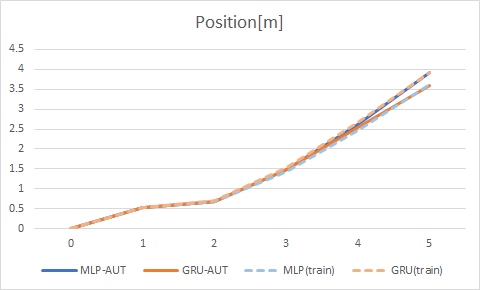
\includegraphics[width=14cm]{./figures/graph_position.png}
\caption{Speed Error Comparison}
\label{fig:graph_position}
\end{center}
\end{figure}

\begin{figure}[H]
\begin{center}
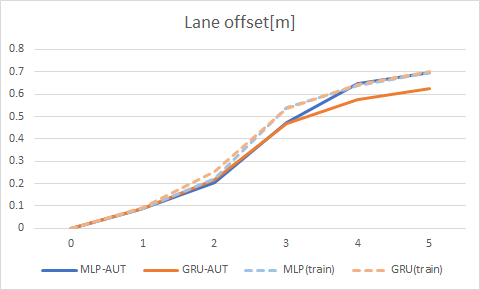
\includegraphics[width=14cm]{./figures/graph_lane.png}
\caption{Speed Error Comparison}
\label{fig:graph_lane}
\end{center}
\end{figure}

\begin{figure}[H]
\begin{center}
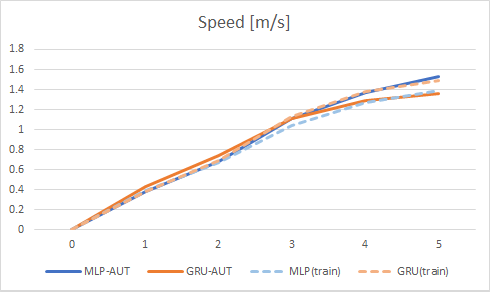
\includegraphics[width=14cm]{./figures/graph_speed.png}
\caption{Speed Error Comparison}
\label{fig:graph_speed}
\end{center}
\end{figure}


\section{Kullback-Leobler Divergence}


\begin{itemize}
\item iTTC
\item Speed
\item Acceleration
\item Turn-Rate
\item Jerk
\end{itemize}

\begin{figure}[H]
\begin{center}
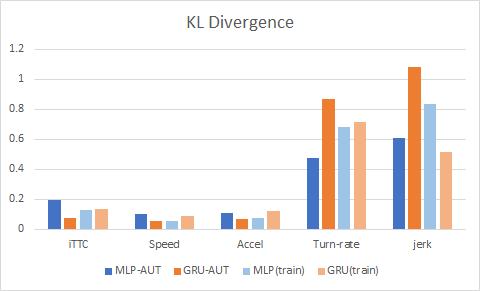
\includegraphics[width=14cm]{./figures/graph_kldivergence.png}
\caption{KL Divergence}
\label{fig:graph_kldivergence}
\end{center}
\end{figure}


\section{Emergent Value}

\begin{itemize}
\item Lane Change Rate
\item Offroad Duration
\item Collision Rate
\item Hard Break Rate
\end{itemize}

\begin{figure}[H]
\begin{center}
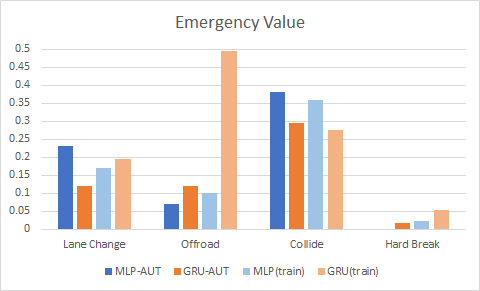
\includegraphics[width=14cm]{./figures/graph_emergency.png}
\caption{Emergent Value}
\label{fig:graph_emergency}
\end{center}
\end{figure}



